\documentclass[UTF8]{article}
\author {Sherlock Liao}
\title {Programming Homework 6}
\usepackage{amsmath}
\usepackage{amssymb}
\usepackage{graphicx}
\begin{document}
\maketitle
\section{Question}
For the question
$$
\begin{cases}
u_t = u_{xx} + y_{yy}, \quad (x,y) \in (0,1) \times (0,1), \quad t > 0 \\
u(x,y,0) = sin(\pi x)sin(2\pi y), \quad (x,y) \in [0,1] \times [0,1] \\
u(0,x,t) = u(1,x,t) = 0, \quad x\in [0,1], t > 0 \\
u(0,y,t) = u(1,y,t) = 0, \quad y\in [0,1], t > 0
\end{cases}
$$
Using FTCS scheme, caculate the function value at t = 0.06, 0.1 and 0.9, compare and discuss the results seperately. $N_x = N_y = 20, \Delta t = 0.0005, 0.001.$

\section{Algorithm}
For FTCS scheme, we partition the space and we can get that
$$
\Delta x = \frac{1}{N_x}, \quad \Delta y = \frac{1}{N_y}
$$
$$
(r,s) \in G = {(r,s), r = 0, 1,\dots, N_x, \quad s = 0, 1, \dots, N_y}
$$
We can get the scheme
$$
v_{r,s}^{n+1} = v_{r,s}^n + \frac{\Delta t}{\Delta x^2}(v_{r+1,s}^n -2v_{r,s}^n + v_{r-1,s}^n) + \frac{\Delta t}{\Delta y^2}(v_{r,s+1}^n-2v_{r,s}^n+v_{r,s-1}^n)
$$
for non-boundary condition.

For boundary condition, this is Dicihelet Boundary Condition. We can get that
$$
v_{0,s}^n = 0 \quad v_{r,0}^n = 0 \quad v_{N_x,s}^n = 0 \quad v_{r, N_y}^n = 0 \quad r=0, 1, \dots, N_x, \quad s = 0, 1, \dots, N_y
$$

\section{Results and Analysis}
\subsection{Results}

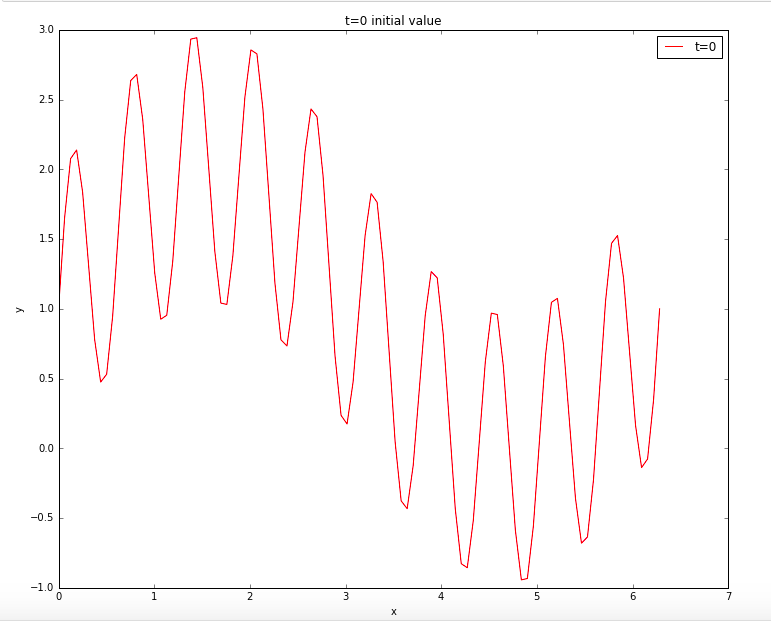
\includegraphics[width=8cm]{1.png}
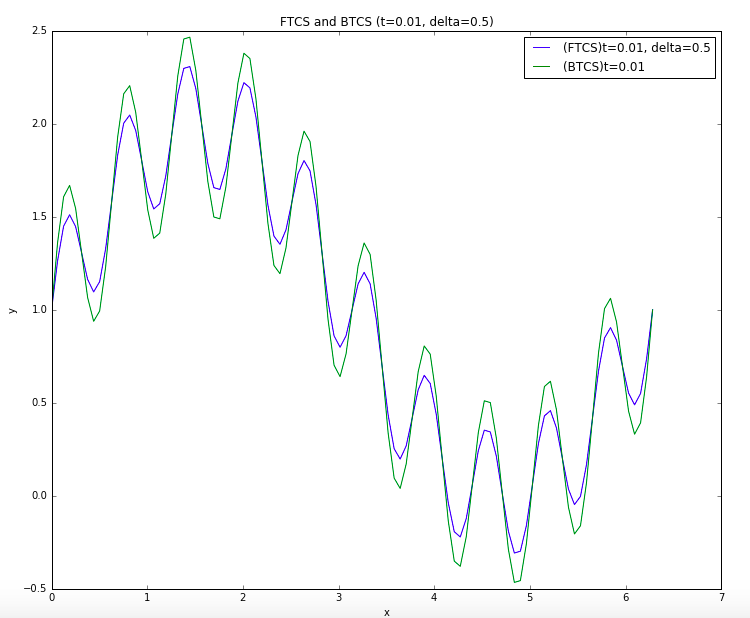
\includegraphics[width=8cm]{2.png}
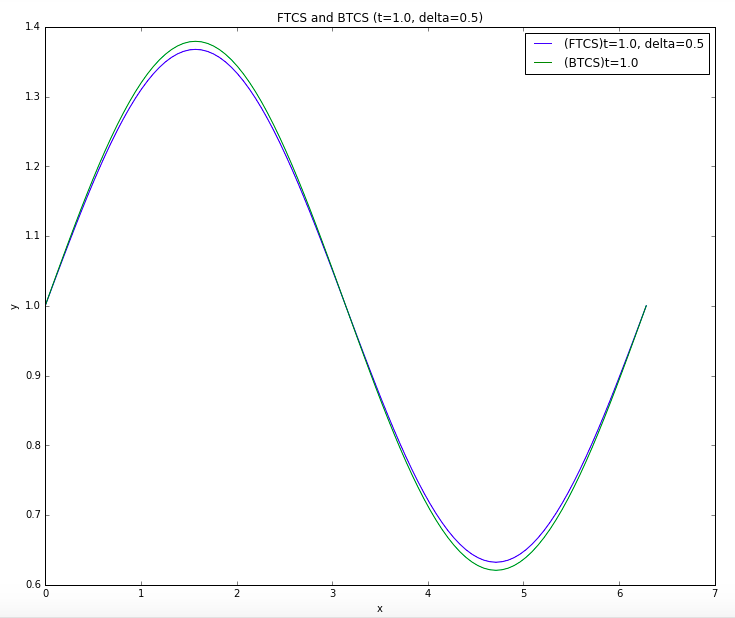
\includegraphics[width=8cm]{3.png}

These three pictures are the values at t=0.06, 0.9 and 0.1 when using $\Delta t = 0.0005$. We can see that the result converge, and the shapes in three picture are almost the same except that the y-coordinate scale is different. It has a very smooth surface. The result is compatible.

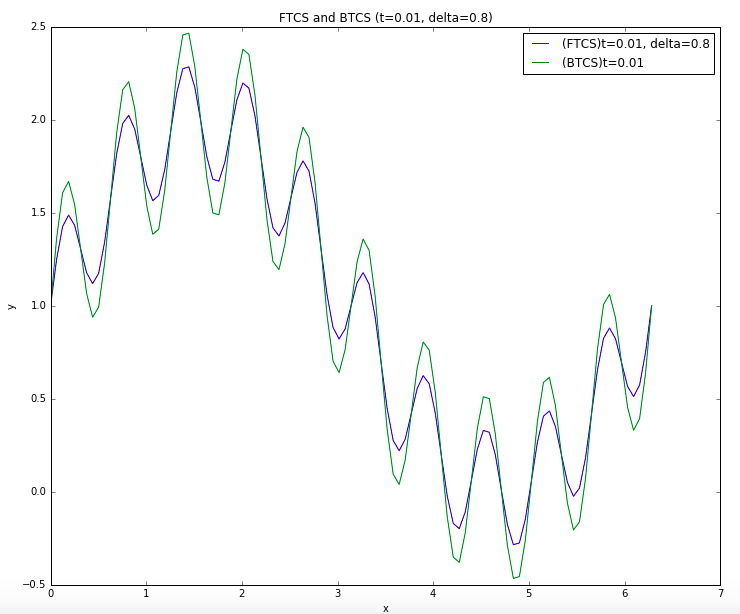
\includegraphics[width=8cm]{4.png}
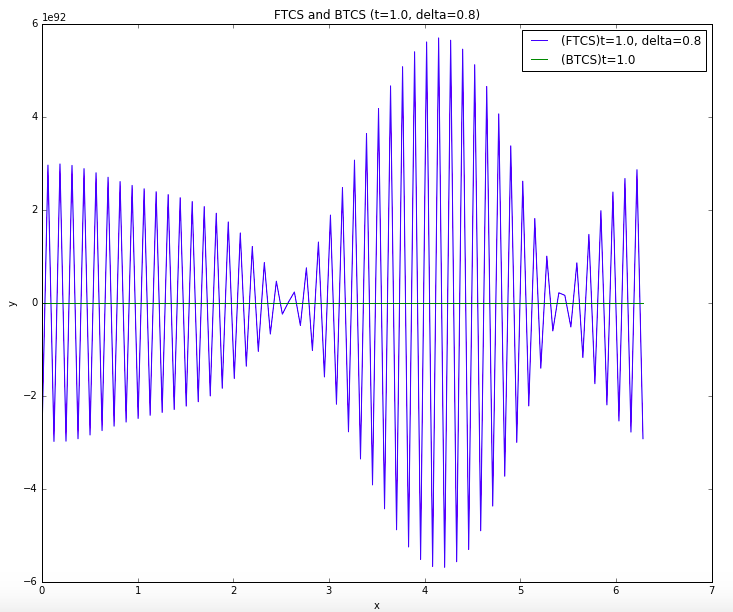
\includegraphics[width=8cm]{5.png}
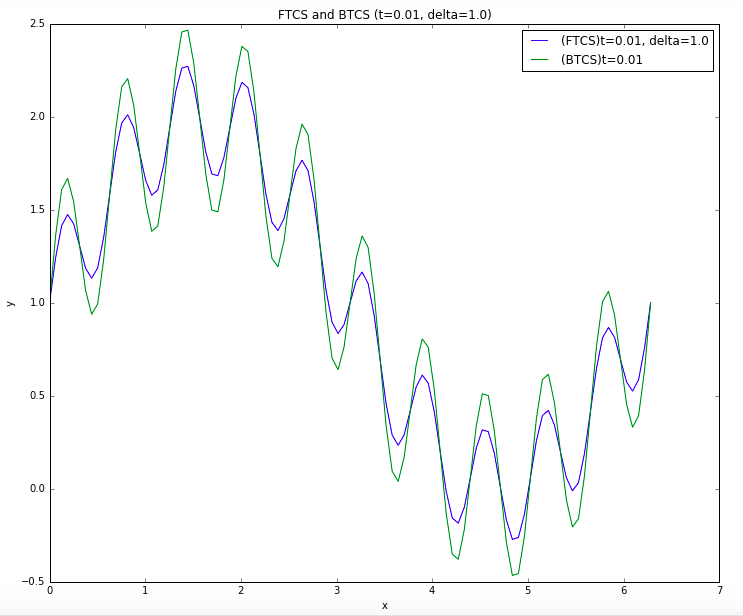
\includegraphics[width=8cm]{6.png}

These three pictures are the values at t=0.06, 0.9 and 0.1 when using $\Delta t =0.001$. The surface is not smooth. As time goes by, it becomes more and more pointed. The result is bad.

\subsection{Analysis}
For FTCS scheme, we consider single wave and we can get $\hat{v}^{n+1} = \hat{Q} \hat{v}^n$. To make it stable, we need to let $|Q| \leq 1$. Then we get that $\frac{\Delta t}{\Delta x^2} + \frac{\Delta t}{\Delta y^2} \leq 1$. Here, we have $\Delta x = \Delta y = \frac{1}{20}$, so we can compute to get $\Delta t \leq 0.00125$. So we can see that if we use $\Delta t = 0.001$ and $\Delta t = 0.0005$ , then $\Delta t = 0.0005$ can get a better result. Because $\Delta t = 0.001$ is more close to 0.00125 than $\Delta = 0.0005$, we can get a better result when $\Delta t = 0.0005$ even we need more time to finish it.









\end{document}
